\chapter{Synthèse de circuits et Quine Mc.Cluskey}
\section{Synthèse des circuits à partir de spécification verbales}
\paragraph{Spécification formelle} Description complète, précise et non-ambiguë de toutes les propriétés d'un système (TdV, K-Map etc.).
\paragraph{Combinatoire} Les sorties du système ne dépendent que des entrées.\\

Si le problème \textbf{est combinatoire}, alors on peut appliquer tout ce qui a été vu jusqu'à présent.\\
N.B. : commencer par déterminer le nombre d'entrées et de sorties
\section{Additionneurs re-visités}
On souhaite réaliser un circuit additionneur de deux mots A et B codés sur 4 bits (peut généraliser pour $n$ bits).\\
deux solutions s'offrent à nous:
\begin{itemize}
	\item Mimer le principe d'addition bit à bit (séquence de calcul dans le temps)
	\item Anticiper le report pour un certain nombre de bits (considérer le problème comme combinatoire)
\end{itemize}
\subsection{Addition bit à bit}
\label{subsec:addbitàbit}
L'addition est faite grâce à:
\begin{itemize}
	\item un 1/2 additionneur (deux opérantes d'un bit, deux bits d'entrées)
	\item $(n-1)\times$ additionneur complet (deux opérantes d'un bit + un bit de report d'une étage précédent, trois bits d'entrées)
\end{itemize}
\begin{minipage}{.45\textwidth}
	\begin{figure}[H]
		\centering
		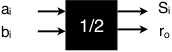
\includegraphics[width=.6\textwidth]{ch5/image1}
	\end{figure}
\end{minipage}
\begin{minipage}{.55\textwidth}
	\begin{figure}[H]
		\centering
		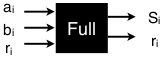
\includegraphics[width=.48\textwidth]{ch5/image2}
	\end{figure}
\end{minipage}
\begin{minipage}[t]{.25\textwidth}
	\begin{table}[H]
		\centering
		$\begin{array}{|c|c|c|c}
			\cline{1-3}
			S_i & 0 & 1 & b_i\\
			\cline{1-3}
			0 & 0 & 1 & \\
			\cline{1-3}
			1 & 1 & 0 & \\
			\cline{1-3}
			\multicolumn{1}{c}{a_i} & \multicolumn{1}{c}{ } & \multicolumn{1}{c}{ }		
		\end{array}$
		\begin{align*}
			S_i &=a_i'b_i+a_ib_i'\\
			&= a_i  \oplus b_i
		\end{align*} 
	\end{table}

\end{minipage}
\begin{minipage}[t]{.2\textwidth}
	\begin{table}[H]
		\centering
		$\begin{array}{|c|c|c|c}
			\cline{1-3}
			r_0 & 0 & 1 & b_i\\
			\cline{1-3}
			0 & 0 & 0 & \\
			\cline{1-3}
			1 & 0 & 1 & \\
			\cline{1-3}
			\multicolumn{1}{c}{a_i} & \multicolumn{1}{c}{ } & \multicolumn{1}{c}{ }		
		\end{array}$
		\begin{equation*}
			r_0 = a_ib_i
		\end{equation*} 
	\end{table}
\end{minipage}
\begin{minipage}[t]{.3\textwidth}
	\begin{table}[H]
		\centering
		$\begin{array}{|c|c|c|c|c|c}
			\cline{1-5}
			S & 00 & 01 & 11 & 10 & a_ib_i\\
			\cline{1-5}
			0 & 0 & 1 & 0 & 1 & \\
			\cline{1-5}
			1 & 1 & 0 & 1 & 0 & \\
			\cline{1-5}
			\multicolumn{1}{c}{r_i} & \multicolumn{1}{c}{ } & \multicolumn{1}{c}{ } & \multicolumn{1}{c}{ } & \multicolumn{1}{c}{ } & \multicolumn{1}{c}{ } 	
		\end{array}$
		\begin{equation*}
			S = a_i\oplus b_i\oplus r_i
			\end{equation*} 
	\end{table}
\end{minipage}
\begin{minipage}[t]{.3\textwidth}
	\begin{table}[H]
		\centering
		$\begin{array}{|c|c|c|c|c|c}
			\cline{1-5}
			r & 00 & 01 & 11 & 10 & a_ib_i\\
			\cline{1-5}
			0 & 0 & 0 & 1 & 0 & \\
			\cline{1-5}
			1 & 0 & 1 & 1 & 1 & \\
			\cline{1-5}
			\multicolumn{1}{c}{r_i} & \multicolumn{1}{c}{ } & \multicolumn{1}{c}{ } & \multicolumn{1}{c}{ } & \multicolumn{1}{c}{ } & \multicolumn{1}{c}{ } 	
		\end{array}$
		\begin{equation*}
			r = a_ib_i+r_ib_i+r_ia_i
		\end{equation*} 
	\end{table}
\end{minipage}
Ainsi, pour un additionneur complet sur 4 bits:
\begin{figure}[H]
	\centering
	
\includegraphics[scale=0.7]{ch5/image3}
\end{figure}
Le problème de ce système est la propagation du report entre les étages: le résultat final sera obtenu après la propagation du report à travers tous les étages de l’additionneur ($n$-délais).
\subsection{Additionneur \textit{Carry Look Ahead} (CLA)}
Le principe est de faire de faire un additionneur complet en un seul circuit combinatoire, permettant d'éviter le problème de délais du à la propagation du report en l'anticipant(\textit{Carry Look Ahead}).\\
Le problème étant combinatoire avec 4 entrées (4 bits) et 3 sorties ($(11)_2+(11)_2=(110)_2$), nous pouvons faire nos K-Maps:\\
\begin{figure}[H]
	\centering
	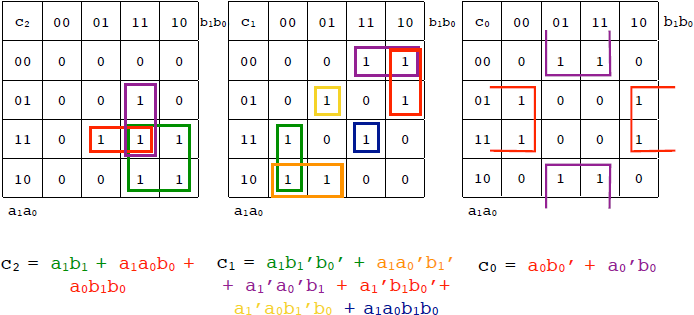
\includegraphics[width=\textwidth]{ch5/image4}
\end{figure}
Pour un plus grand nombre de bits (32, 64 etc.), on préfère mettre en série car si $\nearrow$ entrées/sorties $\rightarrow \nearrow$ taille du circuit (mémoire) $\Rightarrow$ explosion combinatoire.\\
Il y aura un délai de report du à la mise en série, mais moindre que le système vu en \autoref{subsec:addbitàbit}
\section{Encodeurs de priorité}
Un mot D est codé sur $n$ bits. On veut connaître l'index du bit de poids le plus fort ayant un «1» et signaler la présence d'un 1 par un signal ANY.\\

Pour un mot à 4 bits:
\begin{itemize}
	\item 4 entrées
	\item 3 sorties:
	\begin{itemize}
		\item 2 bits pour coder l'index (index max $=4$) 
		\item 1 bit pour le ANY
	\end{itemize}
\end{itemize}
\begin{figure}[H]
	\centering
	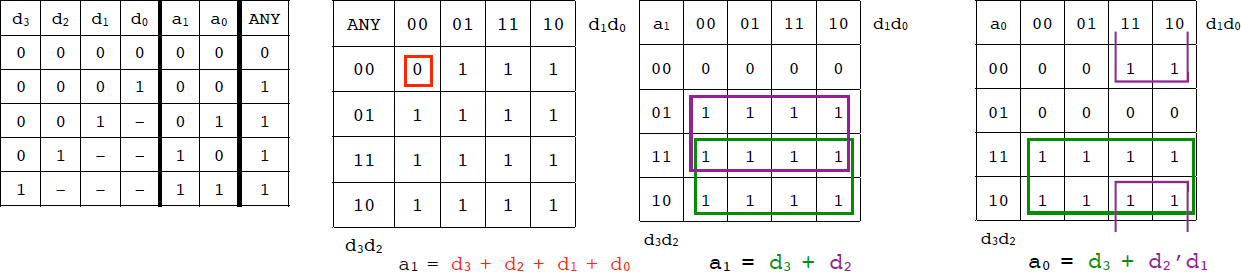
\includegraphics[width=\textwidth]{ch5/image5}
\end{figure}
\section{Simplification des fonctions : Méthode Quine-Mc.Cluskey}
La méthode de Quine-Mc.Cluskey est:
\begin{itemize}
	\item méthode systématique, analysant toutes les possibilités de regroupement. 
	\item utilisée pour un grand nombre de variables
	\item garantit la meilleure solution
	\item facilement programmable
\end{itemize}
Elle se base sur 2 étapes:
\begin{enumerate}
	\item Recherche des implicants premiers  par la \textbf{méthode des tris successifs} (phase d'\textbf{analyse})
	\item Couverture de la fonction  par un choix des implicants premiers (phase de \textbf{synthèse})
\end{enumerate}
\subsection{Étape 1: Analyse}
\label{subsec:analyse}
Elle consiste en 9 étapes (oui, dans le cours c'est 11):
\begin{enumerate}
	\item Pour une fonction $f$ de $n$ variables, on construit $m$ groupements de \textbf{tous les mintermes} de la fonction
	\item Dans chaque groupement des mintermes (noté $G_i$)
	\begin{itemize}
		\item $i$ variables qui valent 1
		\item $(n-i)$ qui valent 0
	\end{itemize}
	\begin{figure}[H]
		\centering
		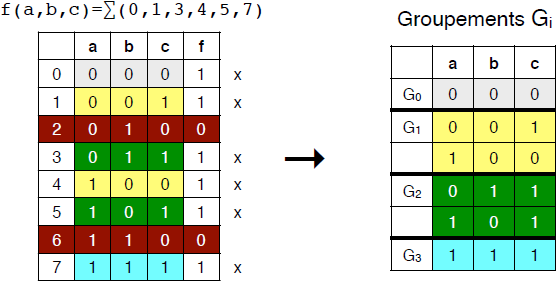
\includegraphics[width=.6\textwidth]{ch5/image6}
	\end{figure}
	\item On compare chaque minterme de $G_i$ avec \textbf{TOUS} les mintermes appartenant à $G_{i+1}$ en termes de la distance de Hamming ($\forall i$)
	\item Si la distance de Hamming entre 2 mintermes $=1$, on les marque par un $x$  et on note \textbf{l'appariement} entre les 2:
	\begin{equation}
		\left.
			\begin{array}{r}
				000\\
				010
			\end{array}
		\right\}\Rightarrow 0\text{-}0
	\end{equation}
	impliquant la possibilité de faire un $n$-cube de plus grande taille (taille 2 à ce stade).\\
	Sinon, il s'agit d'un \textit{impliquant premier} ($n$-cube de taille 1 à ce stade) qu'on notera $IP_k$ dans l'ordre d'apparition
	\item Tous les appariements de $G_i$ et $G_{i+1}$ sont écrits dans un nouveau groupement, noté $G_i'$
	\item Après une première passe, il y a donc au moins $m-1$ groupements $G_i'$
	\item L'ensemble $G_i'$ constitue donc l'ensemble de tous les $n$-cube de taille 2
	\item On répète l'opération avec les nouveaux groupements jusqu'à ce qu'il ne soit plus possible d'apparier
	\item On dresse la liste de tous les implicants premiers (IPs) trouvés.
\end{enumerate}
\subsubsection{Remarques}
\begin{enumerate}
	\item On peut avoir $m=n$
	\item Marquer \textbf{clairement} la séparation entre les $G_i$
	\item Les \textit{don't care} sont également pris en compte pour la distance de Hamming
	\begin{table}[H]
		\centering
		\begin{tabular}{|ccc|}
			\hline
			-000 & Distance de Hamming de 1 & -000\\
			-100 & on \textbf{peut} apparier & -{}-00\\
			\hline
			-000 & Distance de Hamming de 3 & \\
			01-0 & on \textbf{ne peut pas} apparier & \\
			\hline
		\end{tabular}
	\end{table}
	\item S'il y a présence d'indifférent (\textit{don't care}, \textit{don't happen}) au début du problème:
	\begin{itemize}
		\item on fait l'hypothèse qu'ils valent 1 (et donc les rajoutes dans les groupement $G_i$ sans aucune distinction)
		\item Les implicants premiers non-utile (composés que d'indifférents) seront éliminés lors de la 2\up{ème} phase (couverture)
	\end{itemize}
\end{enumerate}
\subsubsection{Exemple}
\begin{equation*}
	f(a,b,c,d,e)=\sum m(0,1,2,5,14,16,18,24,26,30)+\sum d(3,13,28)
\end{equation*}
\begin{figure}[H]
	\centering
	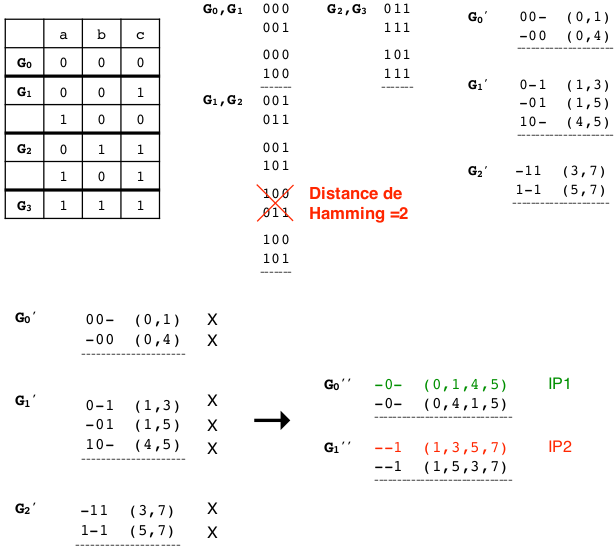
\includegraphics[width=\textwidth]{ch5/image7}
\end{figure}
\begin{figure}[H]
	\centering
	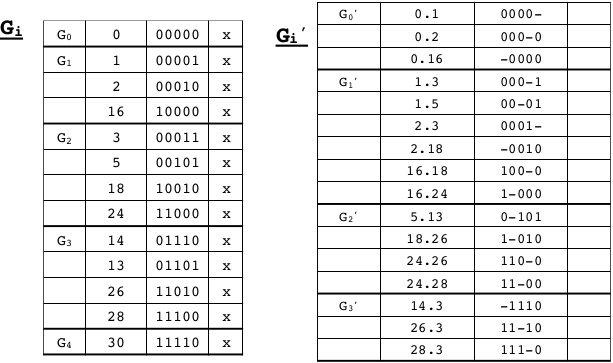
\includegraphics[width=\textwidth]{ch5/image8}
\end{figure}
\begin{figure}[H]
	\centering
	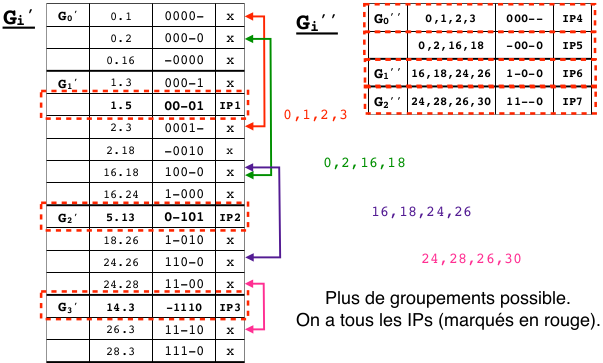
\includegraphics[width=\textwidth]{ch5/image9}
\end{figure}
Ainsi les implicants premiers sont:
\begin{table}[H]
	\centering
	$\begin{array}{ll}
	IP1 & =x_4'x_3'x_1'x_0 \\
	IP2 & =x_4'x_2x_1'x_0\\
	IP3 & =x_3x_2x_1x_0'\\
	IP4 & =x_4'x_3'x_2'\\
	IP5 & =x_3'x_2'x_0'\\
	IP6 & =x_4x_3x_0'\\
	IP7 & =x_4x_2'x_0'\\
	\end{array}$
\end{table}
\subsection{Étape 2 : Couverture de la fonction}
Il existe 2 manières de la faire:
\begin{enumerate}
	\item Via un \textbf{tableau de couverture}:
	\begin{itemize}
		\item méthode graphique
		\item efficace dans certains cas
	\end{itemize}
	\item Via une \textbf{équation de couverture}:
	\begin{itemize}
		\item méthode algébrique
		\item efficace dans tous les cas mais plus de boulot
		\item génère toutes les solutions possibles
	\end{itemize}
\end{enumerate}
\subsubsection{Tableau de couverture}
On dresse un tableau consisté des :
\begin{itemize}
	\item mintermes pour les lignes
	\item implicants premiers pour les colonnes (\textit{C.f.} \autoref{subsec:analyse})
\end{itemize}
Ensuite, pour chaque $IP$ il faut marquer \textbf{tous les mintermes} qu'il permet de couvrir. Enfin, les implicants qui sont les \textbf{seuls} à couvrir un minterme sont des implicants premiers essentiels (il n'est plus nécessaire de couvrir des mintermes déjà couvert).\\

Le problème survient lorsque nous avons le choix de l'$IP$ pour la couverture d'un minterme. Comme nous avons un choix à faire, on aura une combinaison de solution possible. Cette combinaison est "chiante" a trouvé graphiquement, c'est pourquoi nous aurons recourt à l'équation de couverture.

\paragraph{Remarque:} Comme les indifférents ne sont pas représentés dans le tableau, les implicants premiers composés uniquement d'indifférents sont supprimés
\paragraph{Exemple:}
\begin{equation*}
	f(x_4,x_3,x_2,x_1,x_0)=\sum m(0,1,2,5,14,16,18,24,26,30)+\sum d(3,13,28)
\end{equation*}
\begin{figure}[H]
	\hspace{-1.5cm}
	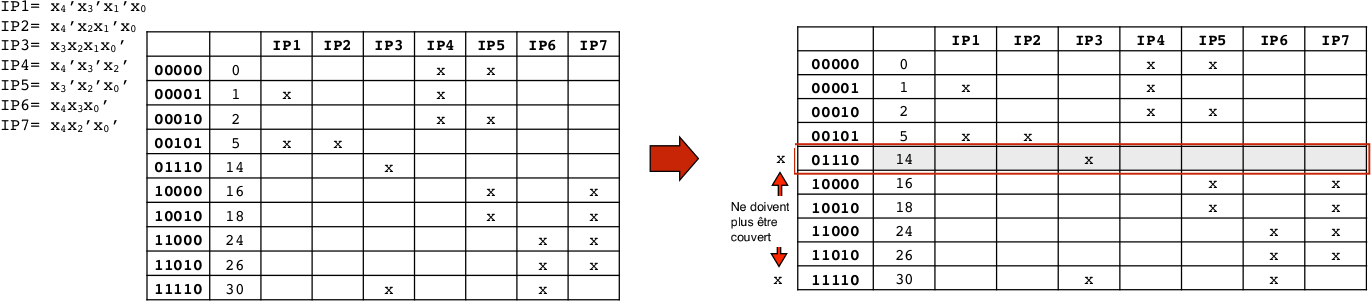
\includegraphics[width=1.2\textwidth]{ch5/image10}
	\caption{Tableau de couverture}
	\label{fig:tableaucouverture}
\end{figure}
\subsubsection{Équation de couverture}
Convertissons les informations graphiques en algébriques. Lorsque nous avons le choix entre plusieurs implicants premiers, ils seront joints par un \textbf{OU}, c-à-d si l'on a le choix entre l'implicant $IP_a$ et $IP_b$ pour un même minterme, on notera $(i_a+i_b)$ (traduction: $IP_a$ ou $IP_b$)\\
\danger on utilise des minuscule pour ne pas confondre avec les $IPs$\\

Il faut faire ceci pour chaque minterme. Comme il faut couvrir tous les mintermes, on lie les différentes expression de couverture pour chaque mintermes par un \textbf{ET} et l'on impose que cette expression doit valoir 1 (par définition). Par exemple, à partir du tableau de la \autoref{fig:tableaucouverture}:
\begin{equation}
	1=(i_4+i_5)(i_1 +i_4)(i_4+i_5)(i_1+i_2)i_3(i_5+i_7)(i_5+i_7)(i_6+i_7)(i_6+i_7)(i_3+i_6)
\end{equation}
Que l'on peut bien évidement simplifier
\begin{equation}
	1=(i_4+i_5)(i_1 +i_4)\cancel{(i_4+i_5)}(i_1+i_2)i_3(i_5+i_7)\cancel{(i_5+i_7)}(i_6+i_7)\cancel{(i_6+i_7)}\cancel{(i_3+i_6)}
\end{equation}
Les termes isolés ($i_3$) sont des implicants essentiels.\\
Ensuite, il suffit de distribuer au maximum tout en simplifiant lorsque cela est possible (petit exercice). On obtient
\begin{equation}
	1=\underbrace{i_3i_4i_1i_7}_{F_1}+\underbrace{i_3i_1i_5i_6}_{F_2}+\underbrace{i_3i_2i_4i_7}_{F_3}+\underbrace{i_3i_2i_4i_5i_6}_{F_4}
\end{equation}
Chaque terme de la somme est donc un solution possible!\\

Ici, on a 4 solutions ($F_1,F_2,F_3,F_4$). les $i_a$ indique quels implicants premier il faut prendre. Pour le 1\up{er} ($F_1$), on doit prendre $IP_3$ et $IP_4$ et $IP_1$ et $IP_7$. Mais l'expression finale est une \textbf{somme} des implicants. Donc on a pour $F_1$:
\begin{equation}
	F_1=IP_3+IP_4+IP_1+IP_7
\end{equation}
Il suffit de remplacer les IPs par leurs véritables expressions (ex: $x_4x_2'x_1$).\\

Néanmoins, on peut encore faire un tri. On ne garde que les expressions contenant le moins de termes $\Rightarrow F_4$ tombe. On a donc, finalement, le choix entre $F_1$, $F_2$ et $F_3$ comme solution. 
\paragraph{fautes graves:}
Les erreurs suivantes sont \textbf{GRAVES}:
\begin{itemize}
	\item Pour la partie analyse:
	\begin{itemize}
		\item Faire des groupements des éléments $G_i$ non-adjacents ($G_i$ et $G_{i+2}$ par exemple).
		\item Ne pas considérer l'hypothèse pour les indifférents.
		\item Considérer toutes les combinaisons des variables (au lieu des mintermes) et obtenir un 1 à la fin (on ne se rend pas compte de l'erreur).
	\end{itemize}
	\item Pour la partie synthèse/couverture:
	\begin{itemize}
		\item Représenter une solution pour la fonction logique comme un ET des implicants premiers au lieu d'un OU.
	\end{itemize}
\end{itemize}
\section{Problème des aléas}
Jusqu'à présent, nous avons considéré que le temps de commutations des portes logiques est nul. La réalité est toute autre, engendrant quelques problèmes, comme celui des aléas.
\subsection{Temps de commutation}
Le temps de commutation est défini comme \textit{le temps moyen nécessaire à ce que le changement à l’entrée provoque le changement de la sortie}.\\

Les circuits logiques (numériques) sont réalisés avec des circuits analogiques $\Rightarrow$ l'instantané n'existe pas!
\begin{figure}[H]
	\centering
	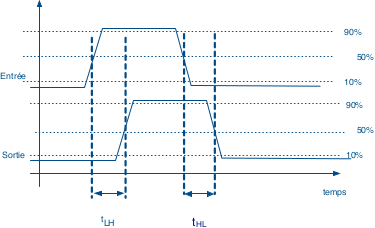
\includegraphics[width=.6\textwidth]{ch5/image11}
	\caption{temps de commutation}
	\label{fig:tempscommutation}
\end{figure}

\subsection{Glitch}
\subsubsection{Introduction}
Introduisons la notion de glitch (ou aléa) par  un exemple simple dans lequel on décide de changer les valeurs des variables d'entrées:
\begin{figure}[H]
	\centering
	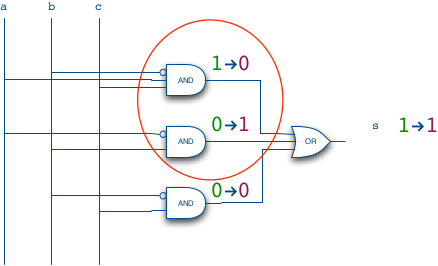
\includegraphics[width=.6\textwidth]{ch5/image12}
\end{figure}
Représentons les changements de valeurs des différentes portes en fonction du temps (temps de commutation non nul)
\begin{figure}[H]
	\centering
	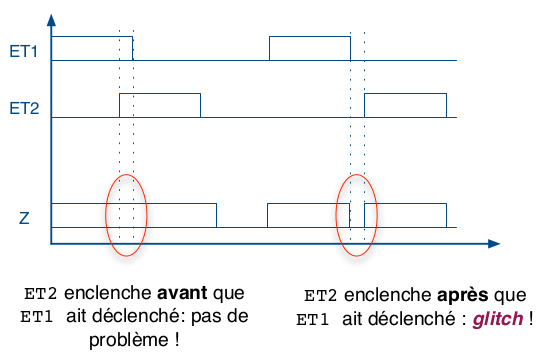
\includegraphics[width=.8\textwidth]{ch5/image13}
	\caption{Glitch}
\end{figure}
\subsubsection{Définition et problématique}
Du coup, définissons ce qu'est un glitch: \textit{un glitch est une impulsion de courte durée non-désirée}.\\

Le problème avec les glitchs est que (comme représenté sur la \autoref{fig:tempscommutation}) on peut obtenir (pendant un court instant) une valeur contraire à ce que l'on attend.\\
Si le système est insensible aux variations courtes, le glitch n'est pas un problème (genre un afficher 7 segments). Mais si le système l'est, gare aux dégâts\dots\ De manière générale, on essaye d'éviter les glitchs.\\
\subsubsection{Explication et solution}
Une représentation sous forme de K-Map montre bien les endroits susceptibles d'apparition de glitch
\begin{figure}[H]
	\centering
	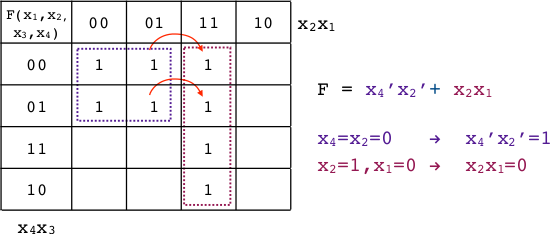
\includegraphics[width=.8\textwidth]{ch5/image14}
\end{figure}
Les endroits susceptibles sont les endroits où l'on passe d'un $n$-cube à un autre.\\

La solution consiste à recouvrir ces «sauts» par un terme redondant, maintenant ainsi la sortie à 1 et évitant donc la possibilité de glitch\\
\begin{minipage}{.5\textwidth}
	\begin{figure}[H]
		\centering
		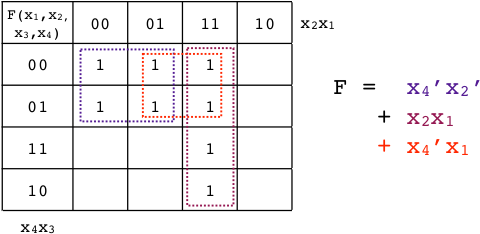
\includegraphics[width=.9\textwidth]{ch5/image15}
	\end{figure}
\end{minipage}
\begin{minipage}{.5\textwidth}
	\begin{figure}[H]
		\centering
		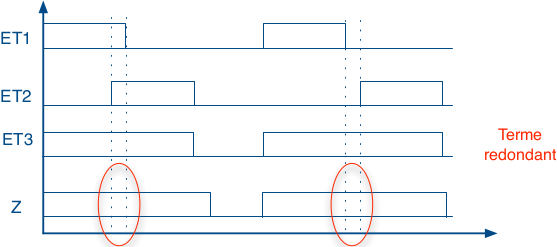
\includegraphics[width=.9\textwidth]{ch5/image16}
	\end{figure}
\end{minipage}